\documentclass[12pt,a4paper]{article}
\usepackage{cmap}
\usepackage[utf8]{inputenc}
\usepackage[T1,T2A]{fontenc}
\usepackage[english,russian]{babel}
\usepackage{array,booktabs,tabularx,amsmath}
\usepackage{caption,float,graphicx,qrcode}
\usepackage{geometry,hyperref,indentfirst,verbatim}
\geometry{margin=25mm}
\hypersetup{unicode=true,colorlinks=true,urlcolor=blue,linkcolor=black}
\setlength{\parindent}{1.25cm}
\setlength{\parskip}{0pt}
\setlength{\emergencystretch}{2em}
\renewcommand{\labelitemi}{\textendash}
\DeclareCaptionLabelSeparator{emdash}{\space---\space}
\captionsetup[figure]{justification=centering,singlelinecheck=false,labelsep=emdash}
\addto\captionsrussian{\renewcommand{\figurename}{Рис.}}
\newcommand{\PositionDocuments}{478\,833}
\newcommand{\PositionTokens}{158\,544\,765}
\newcommand{\PositionCount}{335\,548\,564}
\newcommand{\PositionMB}{2725,12}
\newcommand{\PositionSeconds}{491,30}
\newcommand{\PositionVerifySeconds}{50,90}
\newcommand{\PositionPeakMiB}{335,59}
\newcommand{\PhraseRows}{%
doom AND eternal & 1392 & 1408 & 6,26 & 4,17 \\
\textquotedbl{}doom eternal\textquotedbl{} & 1274 & 1274 & 23,45 & 28,07 \\
\textquotedbl{}eternal doom\textquotedbl{} & 18 & 18 & 7,11 & 7,23 \\
\textquotedbl{}doom eternal\textquotedbl{} AND NOT quake & 1186 & 1186 & 4266,40 & 4029,99 \\
god AND of AND war & 6498 & 7097 & 72,95 & 54,47 \\
\textquotedbl{}god of war\textquotedbl{} & 5804 & 5809 & 432,46 & 424,98 \\
\textquotedbl{}дата выхода\textquotedbl{} & 5682 & 12666 & 72,86 & 137,32 \\
\textquotedbl{}даты выхода\textquotedbl{} & 2819 & 12666 & 38,60 & 134,02 \\
}

\begin{document}
\hypersetup{pageanchor=false}
\begin{titlepage}
\begin{center}
{\large МОСКОВСКИЙ АВИАЦИОННЫЙ ИНСТИТУТ\\
(НАЦИОНАЛЬНЫЙ ИССЛЕДОВАТЕЛЬСКИЙ УНИВЕРСИТЕТ)}
\vspace{18pt}
{\large Факультет информационных технологий и прикладной математики}

{\large Кафедра вычислительной математики и~программирования}
\vfill
{\large\textbf{Лабораторная работа №10 по курсу\\ «Информационный поиск»}}
\vspace{12mm}

{\large\textbf{Цитатный поиск, координаты}}
\vfill
\begin{flushright}
\begin{tabular}{@{}r@{:\hspace{0.6em}}l@{}}
\textit{Студент} & К.\,А. Арусланов\\
\textit{Группа} & М8О-403Б-23\\
\textit{Преподаватель} & А.\,А. Кухтичев\\
\textit{Дата} & 08.11.2026\\
\textit{Оценка} &
\end{tabular}
\end{flushright}
\vfill
Москва, 2026
\end{center}
\end{titlepage}
\hypersetup{pageanchor=true}
\setcounter{page}{2}
\tableofcontents
\newpage

\section{Постановка задачи}
Дополнить поисковую систему координатами слов и цитатным поиском.
Запрос в кавычках должен находить документы, содержащие последовательность
слов в заданном порядке на соседних позициях. Обеспечить сочетание фраз
с булевыми операторами, консольный ввод-вывод и веб-интерфейс.
Основные алгоритмы и структуры данных реализовать самостоятельно на C++.

\section{Метод решения}
\subsection{Зачем нужны координаты}
Булев индекс хранит факт присутствия слова в документе.
Поэтому запрос \texttt{doom AND eternal} удовлетворяется даже тогда,
когда слова находятся в разных предложениях или в обратном порядке.
Список документов не содержит информации, необходимой для проверки фразы.

Координатное расширение сохраняет для каждого термина тройки
$(d,f,p)$: документ, поле и позиция токена внутри поля.
Например, текст «doom new eternal» содержит координаты
$p(\texttt{doom})=0$ и $p(\texttt{eternal})=2$.
Он соответствует конъюнкции, но не фразе
\texttt{\textquotedbl doom eternal\textquotedbl}, поскольку разность позиций
равна двум вместо единицы.

Для фразы из $m$ токенов $w_0,\ldots,w_{m-1}$ требуется
\[
\exists(d,f,p):\quad(d,f,p+i)\in C(w_i),\qquad 0\leq i<m,
\]
где $C(w)$ --- множество координат слова. Иными словами,
нужно найти общую начальную позицию в одном документе и поле.

\subsection{Корпус и представление данных}
Используется снимок корпуса ЛР7--ЛР8 из \PositionDocuments{} документов.
Индексируются заголовок и основной текст. Позиции нумеруются от нуля
отдельно в каждом поле; совпадение через границу полей исключается.
Слова нормализуются тем же токенизатором, что и в предыдущих работах.
Регистр и пунктуация не являются самостоятельными условиями совпадения.
Таким образом, цитатный поиск проверяет последовательность нормализованных
токенов, а не побайтовое равенство исходной строки.

К существующему булевому индексу добавлены два файла.
Первый сопоставляет номеру термина смещение и длину списка координат,
по 16 байт на запись. Второй хранит сами координаты, по 8 байт
на вхождение: 32-битный порядковый номер документа и 32-битное
представление поля и позиции. Старший бит второго числа задаёт поле,
остальные 31 бит --- позицию токена.

Порядковый номер документа переводится в исходный 64-битный ID
через таблицу базового индекса. Это сохраняет поддержку ID с пропусками
и значений больше $2^{32}$. Формат координат ограничен числом документов
не более $2^{32}-1$, числом терминов не более $2^{32}-2$ и позициями меньше
$2^{31}$ в одном поле. Превышения явно отклоняются.

Заголовки файлов содержат версию формата, размеры, контрольные суммы,
отпечатки корпуса, словаря и заголовков базового индекса.
При построении исходный поток проверяется по ID, числу документов
и полной контрольной сумме. Незавершённые файлы и расширение,
относящееся к другому булевому индексу, не допускаются к поиску.

\subsection{Построение с ограниченным буфером}
Собственная хеш-таблица переводит строковые термины в номера словаря.
Из корпуса последовательно формируются тройки
«термин, порядковый номер документа, поле/позиция».
По мере заполнения буфера они сортируются собственной стабильной
поразрядной сортировкой и записываются во временные части.
Два массива сортировки вместе занимают не более 64 МиБ.
Дополнительная память используется для словарей и текущего поля текста.

Отсортированные части сливаются собственной минимальной кучей.
Одновременно открыто не более 24 входов, поэтому при большом количестве
частей выполняется несколько проходов. Повторяющиеся координаты удаляются.
После завершения промежуточные файлы удаляются, а индекс получает
признак готовности. При записи контролируется резерв свободного места
4,5 ГиБ. Корпус и булев индекс остаются неизменными.

\subsection{Потоковое вычисление фраз}
Для слова с номером $i$ координаты сдвигаются на $-i$:
\[
C_i'=\{(d,f,p-i):(d,f,p)\in C(w_i),\ p\geq i\}.
\]
Пересечение $C_0'\cap\ldots\cap C_{m-1}'$ даёт начала совпадающих фраз.
Потоки упорядочены по документу, полю и позиции. Если текущие ключи
не совпадают, продвигаются потоки с меньшим ключом.
При совпадении документ выдаётся один раз независимо от числа
вхождений фразы. Полные списки и промежуточные результаты
в память не загружаются.

Проверка учитывает повторяющиеся слова: фраза «red red» требует
двух соседних позиций, а не одного наличия термина.
В худшем случае для $m$ слов и списков длины $n_i$ затраты текущей
реализации составляют $O(m\sum_i n_i)$ сравнений ключей.
Дополнительный перебор возможен при объединении альтернативных лемм;
число слов и альтернатив ограничено интерфейсом.

\subsection{Два пространства и интерфейсы}
Словоформы и леммы имеют независимые списки координат,
но общую таблицу документов. В режиме лемм варианты одного
слова объединяются до сдвига координат. Все разборы сохраняют
исходную позицию: «стали» может соответствовать «сталь» и «стать»,
но не создаёт искусственную последовательность из двух слов.
Фраза по леммам допускает разные грамматические формы,
сохраняя требование к порядку и соседству.

Фраза становится листом дерева булевого запроса ЛР8.
Например, \texttt{\textquotedbl doom eternal\textquotedbl\ AND NOT quake}
требует фразу и исключает документы со словом \texttt{quake}.
Консольная утилита получает по одному UTF-8-запросу в строке stdin
и выдаёт JSONL в stdout. Веб-форма передаёт запрос тому же ядру C++
и показывает заголовки со ссылками. Python обслуживает интерфейс
и измерения, не вычисляя поисковые множества.

Сохраняются точный подсчёт совпадений и порядок выдачи по ID.
Для фразы допускается до 64 токенов и 512 координатных потоков.
Синтаксические ошибки, отсутствие координат и превышения ограничений
возвращаются явно. Обычные булевы запросы работают и без расширения.

\section{План и результаты тестирования}
GoogleTest проверяет соседство, прямой и обратный порядок,
границы полей, повторяющиеся слова, несколько вхождений и неизвестные
термины. Проверяются фразы в обоих пространствах и их сочетание
с AND, OR и NOT. Для 14 фраз длиной от одного до трёх слов
в каждом режиме полный список ID сравнивается с независимой
проверкой скользящим окном на восьми текстах.

Словарные примеры проверяют разные русские словоформы
и сохранение неоднозначных лемм на одной позиции.
Проверки CLI охватывают JSON, точное число совпадений
при ограниченной выдаче и продолжение после ошибочной строки.
Проверяются пустой индекс, произвольные 64-битные ID,
непарные кавычки и пустые фразы.

Отдельный корпус создаёт более 24 временных частей и два прохода
слияния. Результат побайтово совпадает с индексом, построенным
при большем буфере. Проверяются усечение и повреждение файлов,
незавершённое построение, чужой корпус и словарь,
защита существующего результата и дисковый резерв.

Успешно выполнены 12 GoogleTest и одна процессная проверка CLI.
Два Python-теста проверяют передачу кавычек и пути координат
в нативную программу, а также отображение ошибки поиска.
Журнал приложен в \path{lab10/tests.txt}.

\section{Результаты на корпусе}
\subsection{Объём и построение}
На \PositionTokens{} исходных токенах сохранено
\PositionCount{} координат в двух пространствах.
Число координат включает альтернативные леммы, поэтому не равно
числу исходных вхождений слов. Координатное расширение занимает
\PositionMB{} МБ дополнительно к индексу ЛР7.

\begin{table}[H]
\centering
\begin{tabularx}{\linewidth}{@{}Xr@{}}
\toprule
Показатель & Значение\\
\midrule
Документы & \PositionDocuments\\
Время построения C++, с & \PositionSeconds\\
Полная проверка расширения, с & \PositionVerifySeconds\\
Пиковый рабочий набор при построении, МиБ & \PositionPeakMiB\\
Координаты и таблица смещений, МБ & \PositionMB\\
\bottomrule
\end{tabularx}
\end{table}

Измерение выполнено в нативной Windows Release-сборке GCC 13.1.0.
Время построения включает предварительную полную проверку булева
индекса, чтение корпуса, морфологию, сортировку и запись.
Приведён один прогон построения; память означает рабочий набор
процесса и не включает системный файловый кеш.

\begin{samepage}
Пример начала координатного списка слова \texttt{doom}:
\begin{small}
\verbatiminput{lab10/coordinates.txt}
\end{small}
\noindent
Каждая строка задаёт ID, поле и номер токена. Одному документу
могут соответствовать несколько строк; это отличает координатный
список от булева списка уникальных ID.
\end{samepage}

\subsection{Сравнение конъюнкции и фразы}
Таблица содержит точные количества совпадений и медианы
трёх повторений в одном процессе каждого режима.
Время C++ включает нормализацию, разбор запроса и получение
всех ID, но исключает загрузку словаря и вывод метаданных.
Файловый кеш между повторениями не очищался.

\begin{table}[H]
\centering
\small
\begin{tabularx}{\linewidth}{@{}Xrrrr@{}}
\toprule
 & \multicolumn{2}{c}{Документы} & \multicolumn{2}{c}{Время, мс}\\
Запрос & Формы & Леммы & Формы & Леммы\\
\midrule
\PhraseRows
\bottomrule
\end{tabularx}
\end{table}

Для одной и той же последовательности слов цитатная выдача
является подмножеством конъюнкции: добавлены ограничения на координаты.
Сравнение обратной последовательности показывает, что порядок
является частью условия. Русские примеры позволяют сопоставить
точные словоформы и грамматически нормализованную фразу.
Количество совпадений не заменяет оценку релевантности:
разметка полного корпуса для этих запросов не выполнялась.

Иллюстрация требования к порядку приведена на
рис.~\ref{fig:god-of-war} и~\ref{fig:war-of-god}.
По словоформам фраза «god of war» встречается в 5804 документах,
в том числе в заголовках публикаций об одноимённой игре.
При перестановке тех же слов в «war of god» результат пуст.
Скриншоты показывают отдельные запуски веб-интерфейса;
показанное на них время не является медианой из таблицы.

\begin{figure}[H]
\centering
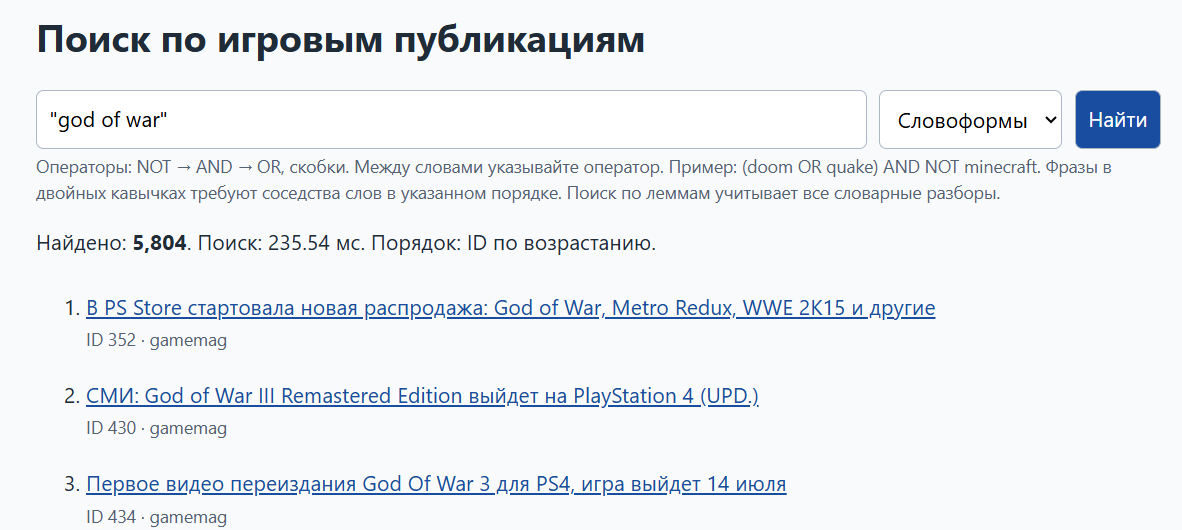
\includegraphics[width=.9\linewidth]{img/god_of_war.png}
\caption{Поиск фразы «god of war» по словоформам: 5804 документа}
\label{fig:god-of-war}
\end{figure}

\begin{figure}[H]
\centering
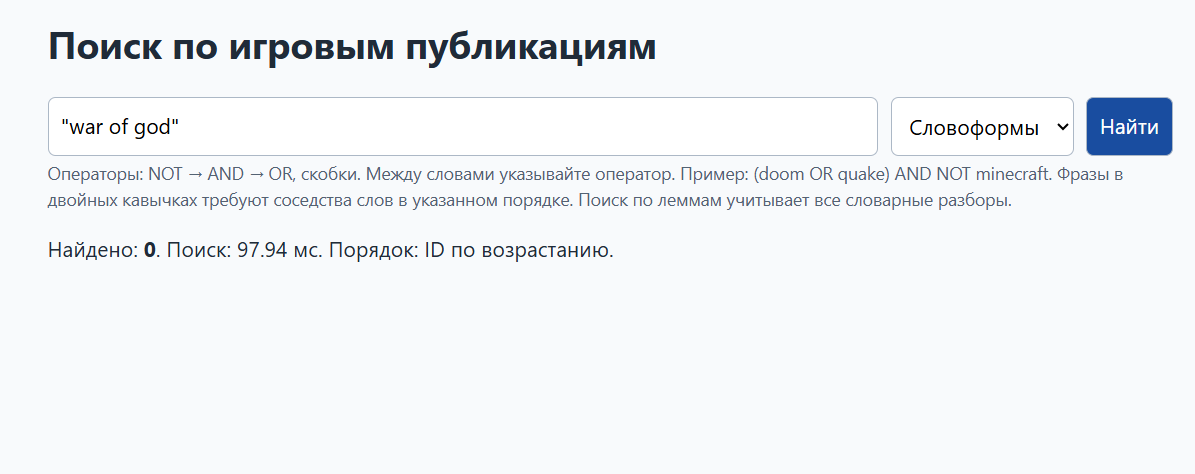
\includegraphics[width=.9\linewidth]{img/war_of_god.png}
\caption{Обратный порядок слов «war of god»: совпадений нет}
\label{fig:war-of-god}
\end{figure}

\subsection{Воспроизводимость}
Скрипт \path{run_lab10.py} запускает тесты, построение,
проверку и пакет запросов \path{tests/fixtures/lab10_queries.txt}.
Сохранены контрольные суммы корпуса, словаря и исполняемых файлов,
исходные JSONL-ответы, повторные времена, статистика памяти
и пример координат. Результаты находятся в \path{doc/lab10/},
инструкция --- в \path{doc/lab10_run.md}.

Исходный код:
\href{https://github.com/kirbasss/MAI-IR/tree/lab10}{github.com/kirbasss/MAI-IR/tree/lab10}.
\begin{figure}[H]
\centering
\begingroup
\hypersetup{urlcolor=black}
\qrcode[height=28mm]{https://github.com/kirbasss/MAI-IR/tree/lab10}
\endgroup
\caption{Ссылка на ветку лабораторной работы №10}
\end{figure}

\section{Вывод}
Реализовано координатное расширение инвертированного индекса
и поиск последовательностей соседних токенов. Общая модель
булевого поиска сохранена: фразы можно соединять логическими
операциями и использовать в отрицании. Раздельная нумерация
полей исключает ложные совпадения через границу заголовка и текста.

Цитатный поиск позволяет выразить требование к устойчивой фразе
или названию, которое невозможно проверить по одному наличию слов.
В режиме лемм требование к координатам сочетается с морфологическим
расширением. Ограничения реализации --- отсутствие сжатия,
прыжков, ранжирования и контекстного снятия омонимии;
пунктуация и границы предложений отдельно не проверяются.
Работа на миллионном корпусе этими измерениями не подтверждается.
Следующие направления развития --- сжатие координат и ускорение
пересечения длинных списков.
\end{document}
